\documentclass[a4paper,12pt]{jlreq}

% 数式関連
\usepackage{amsmath}

% フォント設定(LuaLaTeX または XeLaTeX)
\usepackage{fontspec}
\setmainfont{Latin Modern Roman}

% 数式フォント(unicode-mathを使う場合)
\usepackage{unicode-math}
\setmathfont{Latin Modern Math}

% 画像挿入
\usepackage{graphicx}

% 図表のキャプション調整
\usepackage{caption}

% グラフ作成(PGFPlots)
\usepackage{pgfplots}
\usepgfplotslibrary{statistics}
\pgfplotsset{compat=1.18}

% リンク作成
\usepackage{hyperref}

% 行間
\usepackage{setspace}
\setstretch{1.0}

% ページ余白
\usepackage[top=15mm,bottom=15mm,left=25mm,right=25mm]{geometry}

% 箇条書きスタイル調整
\usepackage{enumitem}



\begin{document}

\title{test}
\author{中村優翔}
\date{\today}
\maketitle

これはテストです。English and math: \( \frac{\sin r}{r} \)
kk
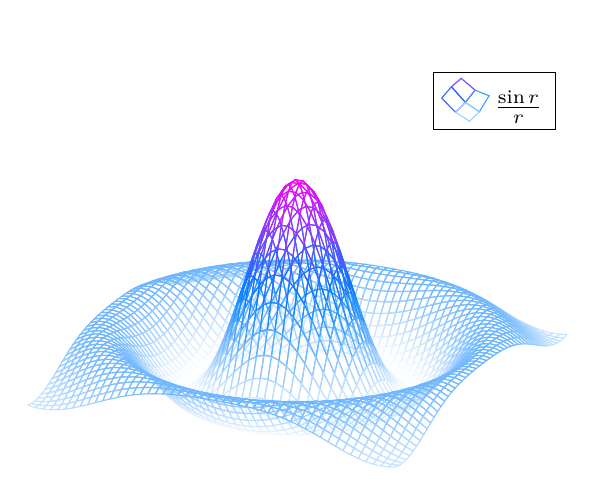
\begin{tikzpicture}
\begin{axis}[
    title=グラフタイトル,
    colormap/cool,
    hide axis,
]
\addplot3[
    mesh,
    samples=50,
    domain=-8:8,
]
{sin(deg(sqrt(x^2+y^2)))/sqrt(x^2+y^2)};
\addlegendentry{$\frac{\sin r}{r}$}
\end{axis}
\end{tikzpicture}

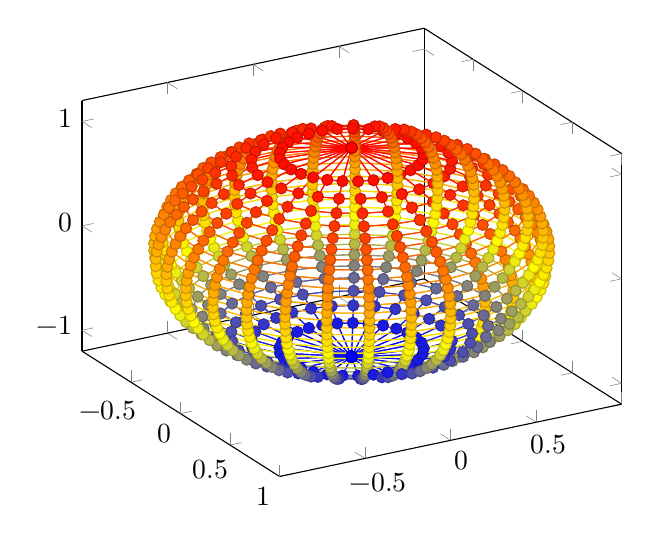
\begin{tikzpicture}
\begin{axis}[view={60}{30}]
\addplot3 [
only marks,
mesh,z buffer=sort,
scatter,scatter src=z,
samples=30,domain=-1:1,y domain=0:2*pi,
] (
{sqrt(1-x^2) * cos(deg(y))},
{sqrt( 1-x^2 ) * sin(deg(y))},
x
);
\end{axis}
\end{tikzpicture}

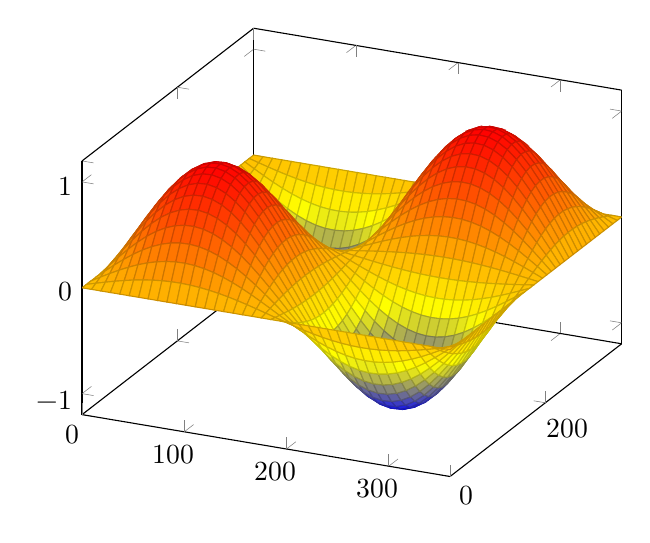
\begin{tikzpicture}
\begin{axis}
\addplot3 [
surf,
domain=0:360,
samples=40,
] {sin(x)*sin(y)};
\end{axis}
\end{tikzpicture}




\end{document}
